\documentclass{beamer}
\usefonttheme[onlymath]{serif}
\usepackage[T1]{fontenc}
\usepackage[utf8]{inputenc}
\usepackage[english]{babel}
\usepackage{amsmath}
\usepackage{amssymb}
\usepackage{amsthm}
\usepackage{gensymb}
\usepackage{parskip}
\usepackage{mathtools}
\usepackage{listings}
\usepackage{hyperref}
\usepackage{graphicx}
\usepackage{color}
\usepackage{enumerate}
\usepackage{tikz}
\usetikzlibrary{calc}
\usetikzlibrary{positioning}
\usetikzlibrary{angles}
\usetikzlibrary{shapes}
\usetikzlibrary{arrows}
\usepackage{verbatim}
\usepackage{multicol}
\usepackage{array}
\usepackage{minted}
\parskip 0pt


\DeclareMathOperator{\lcm}{lcm}
\newcommand\floor[1]{\left\lfloor#1\right\rfloor}
\newcommand\ceil[1]{\left\lceil#1\right\rceil}
\newcommand\abs[1]{\left|#1\right|}
\newcommand\p[1]{\left(#1\right)}
\newcommand\sqp[1]{\left[#1\right]}
\newcommand\cp[1]{\left\{#1\right\}}
\newcommand\norm[1]{\left\lVert#1\right\rVert}
\renewcommand\Im{\operatorname{Im}}
\renewcommand\Re{\operatorname{Re}}

\usetheme{metropolis}
\definecolor{dark yellow}{rgb} {0.6,0.6,0.0}
\definecolor{dark green}{rgb} {0.0,0.6,0.0}

\graphicspath{{myndir/}}

\title{Data Structures}
\author{Arnar Bjarni Arnarson}
\institute{\href{http://ru.is/td}{School of Computer Science} \\[2pt] \href{http://ru.is}{Reykjavík University}}
\titlegraphic{\hfill
\includegraphics[height=0.6cm]{kattis}}

\begin{document}
\maketitle

\begin{frame}[plain]{Today's material}
    \begin{itemize}
        \item Prerequisites
        \item Sliding Window
        \item Heap
        \item Union-Find
        \item Precomputations like prefix sums
        \item Square root decomposition
        \item Segment trees
        \item Sparse tables
    \end{itemize}
\end{frame}

\section*{Prerequisites}

\begin{frame}[plain]
    We assume you know how to implement the following data structures using only fixed size arrays and pointers/objects:
    \begin{itemize}
        \item Dynamically sized arrays (like vector in C++)
        \item Singly/doubly linked lists (like list in C++)
        \item Queue and stack using either of the above
    \end{itemize}
    We also assume you have experience using \texttt{(unordered\_)\{map,set\}}
\end{frame}

\section*{Sliding Window}

\begin{frame}[plain]
	\frametitle{A Sum Problem}
	\begin{block}{Problem description}
    	    Write a program that, given an integer array of size $N$, finds the
            contiguous subarray of size $K$ with the highest sum.
    \end{block}

    \vspace{10pt}
    
    \begin{block}{Input description}
            Input consist of two lines.
            The first line contains two space separated integers $N$, the size of the array, where $1 \leq N \leq 10^6$,
    and $K$, the size of the subarrays to consider, where $1 \leq K \leq N$.
            Then second line contains $N$ space separated integers, the values of the array.
            Each value in the array is between $-10^9$  and $10^9$.
    \end{block}

    \vspace{10pt}
    
    \begin{block}{Output description}
            Output one line, the sum of the highest valued contiguous subarray of size $K$.
    \end{block}
\end{frame}

\begin{frame}[plain]
	\frametitle{A Sum Problem}
	\begin{center}
		\begin{tabular}{|l|l|}
            \hline
            {\footnotesize Sample input} & {\footnotesize Sample output} \\
            \hline
            \ttfamily
            10 4 & 39 \\
            17 20 0 1 5 24 8 2 4 1 &  \\
            \hline
        \end{tabular}
    \end{center}
\end{frame}

\begin{frame}[plain, fragile]
    \frametitle{Straightforward Solution}
	\begin{scriptsize}
        \begin{minted}{python}
n, k = map(int, input().split())
arr = list(map(int, input().split()))
highest = float('-inf')
for start in range(n-k+1):
    end = start + k
    total = 0
    for i in range(start, end):
        total += arr[i]
    highest = max((highest, total))
print(highest)
        \end{minted}
    \end{scriptsize}
    \begin{itemize}
        \item<2-> This solution constructs all size $K$ contiguous subarrays.
        \item<3-> What is the time complexity?
        \item<4-> There are $N$ starting points, each construction takes $K$ steps, so $\mathcal{O}(NK)$.
        \item<5-> Too slow!
    \end{itemize}
\end{frame}

\begin{frame}[plain, fragile]
    \frametitle{Wasted Operations}
    \begin{itemize}
        \item<1-> The subarray starting at index $i$ has the sum $a_i + a_{i+1} + \dots + a_{i+k-1}$.
        \item<2-> The subarray starting at index $i+1$ has the sum $a_{i+1} + a_{i+2} + \dots + a_{i+k}$.
        \item<3-> We iterate over the indices $i+1, i+2, \dotsc, i+k-1$ twice.
        \item<4-> What changes between starting at $i$ vs. starting at $i+1$?
        \item<5-> We subtract $a_i$.
        \item<6-> We add $a_{i+k}$.
        \item<7-> A shift from the subarray starting at $i$ to the subarray starting at $i+1$ takes $\mathcal{O}(1)$ time.
        \item<8-> This is known as the sliding window technique, in this case with a fixed window size.
    \end{itemize}
\end{frame}

\begin{frame}[plain, fragile]
    \frametitle{Sliding Window Solution}
	\begin{scriptsize}
        \begin{minted}{python}
n, k = map(int, input().split())
arr = list(map(int, input().split()))
total = 0
for i in range(k):
    total += arr[i]
highest = total
for i in range(n - k):
    total -= arr[i]
    total += arr[i+k]
    highest = max((highest, total))
print(highest)
        \end{minted}
    \end{scriptsize}
    \begin{itemize}
        \item<2-> What is the time complexity?
        \item<3-> This solution constructs the first size $K$ contiguous subarray.
        \item<4-> Then, $N-K$ times, an element is removed and another added.
        \item<5-> Subtracting and adding numbers is constant time so $\mathcal{O}(N)$.
        \item<6-> Fast enough!
    \end{itemize}
\end{frame}

\begin{frame}[plain]
	\frametitle{A Substring Problem}
	\begin{block}{Problem description}
    	    Write a program that, give a string of size $N$, finds the
            longest substring with $K$ distinct elements.
    \end{block}

    \vspace{10pt}
    
    \begin{block}{Input description}
            Input consist of two lines.
            The first line contains two space separated integers $N$, the size of the string, where $1 \leq N \leq 10^6$,
    and $K$, the number of distinct elements the substring must have, where $1 \leq K \leq 26$.
            Then second line contains a string of length $N$ consisting of English lowercase characters.
    \end{block}

    \vspace{10pt}
    
    \begin{block}{Output description}
            Output one line, the longest substring with $K$ distinct elements.
            If no such string exists, output ``\texttt{DOES NOT EXIST}'', without quotations.
    \end{block}
\end{frame}

\begin{frame}[plain]
	\frametitle{A Substring Problem}
	\begin{center}
		\begin{tabular}{|l|l|}
            \hline
            {\footnotesize Sample input} & {\footnotesize Sample output} \\
            \hline
            \ttfamily
            14 3 & cdcbcbcb \\
            bacdcbcbcbabdb & \\
            \hline
        \end{tabular}
    \end{center}
\end{frame}

\begin{frame}[plain, fragile]
    \frametitle{General Framework}
    \begin{scriptsize}
        \begin{minted}{python}
from string import ascii_lowercase
n, k = map(int, input().split())
s = input()

best_ind, best_len = distinct_k(n, k, s)

if best_len == -1:
  print("DOES NOT EXIST")
else:
  print(s[best_ind:best_ind + best_len])
        \end{minted}
    \end{scriptsize}
\end{frame}

\begin{frame}[plain, fragile]
    \frametitle{Straightforward Solution}
	\begin{tiny}
        \begin{minted}{python}
def distinct_k(n, k, s):
  best_ind, best_len = -1, -1
  for start in range(n):
    for end in range(start, n+1):
      substring = s[start:end]
      distinct = 0
      for symbol in ascii_lowercase:
        if symbol in substring:
          distinct += 1
      cur_len = len(substring)
      if distinct == k and cur_len > best_len:
        best_ind = start
        best_len = cur_len
  return best_ind, best_len
        \end{minted}
    \end{tiny}
    \begin{itemize}
        \item<2-> What is the time complexity?
        \item<3-> There are $\mathcal{O}(N^2)$ substrings of the string
        \item<4-> Checking each one takes us $\mathcal{O}(N)$ time, so $\mathcal{O}(N^3)$ in total.
        \item<5-> Way too slow!
    \end{itemize}
\end{frame}

\begin{frame}[plain, fragile]
    \frametitle{Constant optimization}
	\begin{tiny}
        \begin{minted}{python}
def distinct_k(n, k, s):
  best_ind, best_len = -1, -1
  for start in range(n):
    for end in range(start, n+1):
      substring = s[start:end]
      present = [False for _ in range(26)]
      for symbol in substring:
        present[ord(symbol) - ord('a')] = True
      distinct = sum(present)
      cur_len = len(substring)
      if distinct == k and cur_len > best_len:
        best_ind = start
        best_len = cur_len
  return best_ind, best_len
        \end{minted}
    \end{tiny}
    \begin{itemize}
        \item<2-> This is a little faster, by a factor of $26$ approximately.
        \item<3-> Time complexity is the same.
        \item<4-> Note that \texttt{present} barely differs between adjacent values of \texttt{end}
        \item<5-> Build it as the substring grows.
    \end{itemize}
\end{frame}

\begin{frame}[plain, fragile]
    \frametitle{Incremental}
	\begin{tiny}
        \begin{minted}{python}
def distinct_k(n, k, s):
  best_ind, best_len = -1, -1
  for start in range(n):
    present = [False for _ in range(26)]
    for end in range(start, n):
      present[ord(s[end]) - ord('a')] = True
      distinct = sum(present)
      cur_len = end - start + 1
      if distinct == k and cur_len > best_len:
        best_ind = start
        best_len = cur_len
  return best_ind, best_len
        \end{minted}
    \end{tiny}
    \begin{itemize}
        \item<2-> Now each substring is processed in constant time.
        \item<3-> Time complexity is $\mathcal{O}(N^2)$
        \item<4-> For a given value of \texttt{ind}, adjacent \texttt{start} values have similar values of \texttt{present}.
        \item<5-> Note that adding characters will never decrease \texttt{distinct}.
        \item<6-> However, removing elements from the front may reduce \texttt{distinct}.
    \end{itemize}
\end{frame}


\begin{frame}[plain, fragile]
    \frametitle{Sliding Window}
	\begin{tiny}
        \begin{minted}{python}
def distinct_k(n, k, s):
  best_ind, best_len = -1, -1
  start, end, distinct = 0, 0, 0
  count = [0 for _ in range(26)]
  while start < n:
    while end < n:
      c = ord(s[end]) - ord('a')
      if distinct == k and count[c] == 0:
        break
      count[c] += 1
      end += 1
      distinct = sum(x > 0 for x in count)
    cur_len = end - start
    if distinct == k and cur_len > best_len:
      best_ind = start
      best_len = cur_len
    count[ord(s[start]) - ord('a')] -= 1
    start += 1
    distinct = sum(x > 0 for x in count)
  return best_ind, best_len
        \end{minted}
    \end{tiny}
    \vspace*{-0.3cm}
    \begin{itemize}
        \item<2-> What is the time complexity? \only<3-> { It may seem quadratic at first}
        \item<4-> Each element gets added and removed once, so $\mathcal{O}(N)$.
        \item<5-> Lets introduce $C$, the number of different symbols possible.
        \item<6-> The time complexity is actually $\mathcal{O}(NC)$, but we can do better!
    \end{itemize}
\end{frame}


\begin{frame}[plain, fragile]
    \frametitle{Sliding Window Improved}
	\begin{tiny}
        \begin{minted}{python}
def distinct_k(n, k, s):
  best_ind, best_len = -1, -1
  start, end, distinct = 0, 0, 0
  count = [0 for _ in range(26)]
  while start < n:
    while end < n:
      c = ord(s[end]) - ord('a')
      if distinct == k and count[c] == 0:
        break
      if count[c] == 0:
        distinct += 1
      count[c] += 1
      end += 1
    cur_len = end - start
    if distinct == k and cur_len > best_len:
      best_ind = start
      best_len = cur_len
    c = ord(s[start]) - ord('a')
    count[c] -= 1
    if count[c] == 0:
      distinct -= 1
    start += 1
    distinct = sum(x > 0 for x in count)
  return best_ind, best_len
        \end{minted}
    \end{tiny}
    \begin{itemize}
        \item<2-> Now adding/removing an element is $\mathcal{O}(1)$.
        \item<3-> The time complexity is now $\mathcal{O}(N + C)$.
    \end{itemize}
\end{frame}

\begin{frame}
    \frametitle{General Method}
    \begin{itemize}
        \item<1->  This method is applicable when working with substrings or subarrays.
        \item<2->  The data has to be contiguous, or in other words, no gaps between selected elements.
        \item<3->  Usually you want the maximal or the minimal window fulfilling a certain condition.
    \end{itemize}
\end{frame}

\begin{frame}
    \frametitle{General Method}
    \begin{itemize}
        \item<1->  Suppose that your current window is $[i, j)$ which are both initialized as $0$.
        \item<2->  Define an operation \texttt{add} which adds $a_j$ to your subarray, finally increasing $j$ by $1$.
        \item<3->  Define an operation \texttt{remove} which removes $a_i$ from your subarray, finally increasing $i$ by $1$.
        \item<4->  Step 1: If performing \texttt{add} does not break your condition, perform it and repeat step 1. Otherwise go to step 2.
        \item<5->  Step 2: Check if the current window is a better answer and possibly update. Then go to step 3.
        \item<6->  Step 3: Perform \texttt{remove} and go to step 1.
        \item<7-> Time complexity is $\mathcal{O}(N \cdot (X + Y))$ where $X$ and $Y$ are the cost of \texttt{add} and \texttt{remove}, respectively.
    \end{itemize}
\end{frame}

\section*{Heap}

\begin{frame}[plain]{Heaps}
    \begin{itemize}
        \item<1-> As an example of a data structure in the standard library but that sometimes requires a more powerful version, let us consider heaps.
        \item<2-> Heaps are implemented in most standard libraries in the forms of priority queues.
        \item<3-> A heap is nothing but a binary tree satisfying \textit{the heap condition}.
        \item<4-> The heap condition (for a min heap) says that the value of any given node is not greater than that of its chilren.
    \end{itemize}
\end{frame}

\begin{frame}[plain]{Heaps}
    \begin{itemize}
        \item<1-> Since arrays are linear, we want to smush this binary tree into an array for the implementation.
        \item<2-> We can do this by putting the root at index $1$. Then the children of item at index $i$ are simply at $2i$ and $2i+1$. The parent of any item $i > 1$ is then $\floor{\frac{i}{2}}$.
        \item<3-> We could do this using raw arrays (then index $0$ can be used to store its size), but the examples will be given in C++ using vectors.
    \end{itemize}
\end{frame}

\begin{frame}[plain]{Heaps}
    \begin{center}
    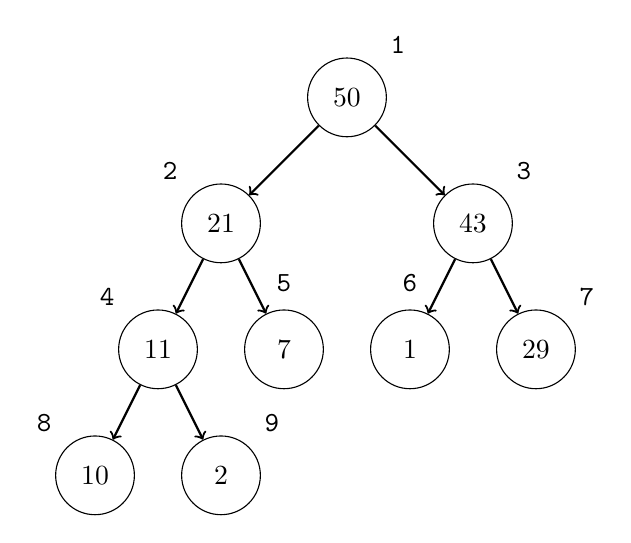
\begin{tikzpicture}[scale=0.8]
    \def\spa{2}
    \node[minimum size=1cm, draw, circle] (A) at (0, 0) {$50$};
    \node[minimum size=1cm, draw, circle] (B) at (-\spa, -\spa) {$21$};
    \node[minimum size=1cm, draw, circle] (C) at (\spa, -\spa) {$43$};
    \node[minimum size=1cm, draw, circle] (D) at (-1.5*\spa, -2*\spa) {$11$};
    \node[minimum size=1cm, draw, circle] (E) at (-0.5*\spa, -2*\spa) {$7$};
    \node[minimum size=1cm, draw, circle] (F) at (0.5*\spa, -2*\spa) {$1$};
    \node[minimum size=1cm, draw, circle] (G) at (1.5*\spa, -2*\spa) {$29$};
    \node[minimum size=1cm, draw, circle] (H) at (-2*\spa, -3*\spa) {$10$};
    \node[minimum size=1cm, draw, circle] (I) at (-\spa, -3*\spa) {$2$};
    
    \node (Ai) [above right=0.1cm of A] {\texttt{1}};
    \node (Bi) [above left=0.1cm of B] {\texttt{2}};
    \node (Ci) [above right=0.1cm of C] {\texttt{3}};
    \node (Di) [above left=0.1cm of D] {\texttt{4}};
    \node (Ei) [above=0.1cm of E] {\texttt{5}};
    \node (Fi) [above=0.1cm of F] {\texttt{6}};
    \node (Gi) [above right=0.1cm of G] {\texttt{7}};
    \node (Hi) [above left=0.1cm of H] {\texttt{8}};
    \node (Ii) [above right=0.1cm of I] {\texttt{9}};
    
    \draw[->, thick] (A) -- (B);
    \draw[->, thick] (A) -- (C);
    \draw[->, thick] (B) -- (D);
    \draw[->, thick] (B) -- (E);
    \draw[->, thick] (C) -- (F);
    \draw[->, thick] (C) -- (G);
    \draw[->, thick] (D) -- (H);
    \draw[->, thick] (D) -- (I);
    \end{tikzpicture}
    \end{center}
    \begin{large}
    \texttt{ARRAY: [SIZE, 50, 21, 43, 11, 7, 1, 29, 10, 2]}
    \end{large}
\end{frame}

\begin{frame}[plain]{Heaps}
    \begin{itemize}
        \item<1->Items can be inserted by pushing them to the back and fixing the heap condition upwards from them.
        \item<2-> Items can be deleted by replacing the smallest value with a leaf and then fixing the heap condition downwards.
        \item<3-> Let us see how this would look in C++.
    \end{itemize}
\end{frame}

\begin{frame}[plain, fragile]{C++ implementation (min-heap)}
    \scriptsize
    \begin{minted}{cpp}
template<typename T> struct Heap {
    vector<T> h; Heap() : h(1) { }
    constexpr size_t size() { return h.size() - 1; }
    constexpr T peek() { return h[1]; }
    void swim(size_t i) {
        while(i != 1 && h[i] < h[i / 2]) {
            swap(h[i], h[i / 2]);
            i /= 2; } }
    void sink(size_t i) {
        while(true) {
            size_t mn = i;
            if(2 * i + 1 < h.size() && h[mn] > h[2 * i + 1]) mn = 2 * i + 1;
            if(2 * i  < h.size() && h[mn] > h[2 * i]) mn = 2 * i;
            if(mn != i) swap(h[i], h[mn]), i = mn;
            else break; } }
    void pop() {
        h[1] = h.back();
        h.pop_back(); sink(1); }
    void push(T x) {
        h.push_back(x);
        swim(h.size() - 1); } };
    \end{minted}
\end{frame}

\begin{frame}[plain]{Heaps}
    \begin{itemize}
        \item<1-> We note that peek and size run in $\mathcal{O}(1)$ while all other operations run in $\mathcal{O}(log(n))$.
        \item<2-> This implementation isn't any better than the standard library one in C++.
        \item<3-> We provide it for demonstration of representing binary trees with an array.
    \end{itemize}
\end{frame}

\section*{Union-Find}

\begin{frame}[plain]{Union-Find}
    \begin{itemize}
        \item<1-> We have $n$ items
        \item<2-> Maintains a collection of disjoint sets (or equivalently, an equivalence relation)
        \item<3-> Each of the $n$ items is in exactly one set
        \item<4-> We represent each set with one of its members, a representative element
        \item<5-> Supports two operations efficiently: \texttt{find(x)} and \texttt{union(x,y)}.
        \item<6-> Operation \texttt{find(x)} finds the representative of the set $x$ is in
        \item<7-> Operation \texttt{union(x, y)} unions the sets of which $x$ and $y$ are members.
    \end{itemize}
\end{frame}

\begin{frame}[plain]{Union-Find}
    \begin{itemize}
        \item<1-> It is generally initialized with all items being in their own set.
        \item<2-> So for $n = 5$ we start out with $\{\{1\},\{2\},\{3\},\{4\},\{5\}\}$.
        \item<3-> \texttt{union(1, 3)} then changes this to $\{\{1, 3\}, \{2\}, \{4\}, \{5\}\}$.
		\item<4-> \texttt{union(2, 5)} then results in $\{\{1, 3\}, \{2, 5\}, \{4\}\}$.
		\item<5-> \texttt{union(2, 4)} then results in $\{\{1, 3\}, \{2, 4, 5\}\}$.
		\item<6-> \texttt{union(1, 4)} finally results in $\{\{1, 2, 3, 4, 5\}\}$.
        \item<7-> At any given point $\texttt{find(x)}$ returns some value in the same set as $x$.
        \item<8-> The important bit is that \texttt{find(x)} returns the same value for all elements of the same set, the representative.
    \end{itemize}
\end{frame}

\begin{frame}[plain]{Union-Find}
    \begin{itemize}
        \item<1-> We can do this by maintaining an array of parents, letting the $i$-th value be the index of the parent of the $i$-th item.
        \item<2-> If a value has no parent, we can denote this somehow, make it its own parent, give it the value $-1$, exactly what we do is not important.
        \item<3-> To get the representative of $x$ we go to the parent of our current item (starting at $x$) until the item has no parent.
        \item<4-> Then to unite $x, y$ we simply make the representative of $x$ the parent of the representative of $y$.
    \end{itemize}
\end{frame}

\begin{frame}[plain,fragile]{Naïve Union-Find implementation}
    \begin{minted}{cpp}
struct union_find {
    vector<int> parent;
    union_find(int n) {
        parent = vector<int>(n);
        for(int i = 0; i < n; i++) {
            parent[i] = i;
        }
    }
    int find(int x) {
        return parent[x] == x ? x : find(parent[x]);
    }
    void unite(int x, int y) {
        parent[find(x)] = find(y);
    }
};
    \end{minted}
\end{frame}

\begin{frame}[plain]{Union-Find}
    \begin{itemize}
        \item<1-> The problem here is that for specific queries, the parent chains may end up being of length $\mathcal{O}(n)$, making each query linear.
        \item<2-> The key to making this more efficient is making those chains shorter.
        \item<3-> One method is to use what is known as small-to-large merging, where the smaller group's leader is made to point to the larger group's leader.
        \item<4-> This ensures the height increases by $1$ as a group's size doubles, resulting in $\mathcal{O}(\log n)$ complexity.
        \item<5-> We can also do this by flattening the chain each time we query \texttt{find}, so the amortized complexity becomes good.
        \item<6-> Here the worst case is still $\mathcal{O}(n)$ but the amortized complexity is $\mathcal{O}(\alpha(n))$ which may as well be a constant, as it is $<5$ for $n$ equal to the number of atoms in the observable universe.
    \end{itemize}
\end{frame}

\begin{frame}[plain,fragile]{Path compressed Union-Find implementation}
    \begin{minted}{cpp}
struct union_find {
    vector<int> parent;
    union_find(int n) {
        parent = vector<int>(n);
        for (int i = 0; i < n; i++) {
            parent[i] = i;
        }
    }
    int find(int x) {
        if(parent[x] == x) return x;
        return parent[x] = find(parent[x]);
    }
    void unite(int x, int y) {
        parent[find(x)] = find(y);
    }
};
    \end{minted}
\end{frame}

\begin{frame}[plain]{Union-Find applications}
    \vspace{30pt}
    \begin{itemize}
        \item<1-> Union-Find maintains a collection of disjoint sets
        \item<2-> When are we dealing with such collections?
        \item<3-> Usually when we want to work with equivalence relations like graph connectivity
        \item<4-> By modifying the data structure it can also contain more queryable data
        \begin{itemize}
            \item<5-> Number of different sets currently
            \item<6-> Current size of the set containing $x$
            \item<7-> An iterable list of all elements of the set containing $x$
        \end{itemize}
        \item<8-> When tracking size you can use it to always perform small-to-large merges for $\mathcal{O}(\log n)$ time complexity.
    \end{itemize}
\end{frame}

\begin{frame}[plain]{Example problem: Skolavslutningen}
    \begin{itemize}
        \item https://open.kattis.com/problems/skolavslutningen
    \end{itemize}
\end{frame}

\section*{Range Queries}

\begin{frame}[plain]{Range queries}
    \vspace{30pt}
    \begin{itemize}
        \item<1-> We have an array $A$ of size $n$.
        \item<2-> Given $i,j$, we want to answer:
            \begin{itemize}
                \item<3-> $\mathrm{max}(A[i],A[i+1],\ldots,A[j-1],A[j])$
                \item<4-> $\mathrm{min}(A[i],A[i+1],\ldots,A[j-1],A[j])$
                \item<5-> $\mathrm{sum}(A[i],A[i+1],\ldots,A[j-1],A[j])$
            \end{itemize}
        \item<6-> We want to answer these queries efficiently, or in other words, without looking through all elements.
        \item<7-> Sometimes we also want to update elements.
    \end{itemize}
\end{frame}

\subsection*{Range sum on constant array}

\begin{frame}[plain]{Range sum on constant array}
    \begin{itemize}
        \item<1-> Let's look at range sums on a constant array
        \item<2-> How do we support these queries efficiently?
    \end{itemize}

    \only<3-> {
    \begin{itemize}
        \item<3-> Simplification: only support queries of the form $\mathrm{sum}(0, j)$
        \item<4-> Notice that $\mathrm{sum}(i,j) = \mathrm{sum}(0,j) - \mathrm{sum}(0,i-1)$
    \end{itemize} }
\end{frame}

\begin{frame}[plain]{Range sum on a static array}
    \begin{itemize}
        \item<1-> So we're only interested in prefix sums
        \item<2-> But there are only $n$ of them...
        \item<3-> Just compute them all once in the beginning
    \end{itemize}
    \vspace{10pt}
    
    \only<4->{
    \begin{center}
        \begin{tabular}{|c|c|c|c|c|c|c|}
            \hline
            1 & 0 & 7 & 8 & 5 & 9 & 3 \\
            \hline
            \onslide<5->{1} & \onslide<6->{1} & \onslide<7->{8} & \onslide<8->{16} & \onslide<9->{21} & \onslide<10->{30} & \onslide<11->{33} \\
            \hline
        \end{tabular}
    \end{center} }

    \begin{itemize}
        \onslide<12->{\item $O(n)$ time to preprocess}
        \onslide<13->{\item $O(1)$ time each query}

        \vspace{10pt}
        \onslide<14->{\item Can we support updating efficiently? \onslide<15->{No, at least not without modification}}
    \end{itemize}
\end{frame}

\begin{frame}[plain]{Generalizing}
    \begin{itemize}
        \item<1-> This works on any invertible function.
        \item<2-> If we want the product we can store the products and use $\mathrm{mul}(i,j) = \mathrm{mul}(0,j) / \mathrm{mul}(0,i-1)$.
        \item<3-> This also works for multidimensional arrays, but the math is more involved.
        \item<4-> We let $\mathrm{sum}(x_i,x_j,y_i,y_j)$ denote the query for the sum from $x_i$ to $x_j$ along the $x$-dimension, and the same for $y$.
        \item<5-> Then the formula becomes
        \begin{align*}
            \mathrm{sum}(x_i,x_j,y_i,y_j) &= \mathrm{sum}(0,x_j,0,y_j) \\
                                          &- \mathrm{sum}(0,x_{i-1},0,y_j) \\
                                          &- \mathrm{sum}(0,x_j,0,y_{i-1}) \\
                                          &+ \mathrm{sum}(0,x_{i-1},0,y_{i-1})
        \end{align*}
    \end{itemize}
\end{frame}

\begin{frame}[plain]{2D sum}
    \begin{center}
        \begin{tikzpicture}
            \draw[step=1,black,thin] (0,0) grid (6,6);
            \node at (-0.1, 5.5) {\tiny \texttt{0}};
            \node at (-0.1, 4.5) {\tiny \texttt{1}};
            \node at (-0.1, 3.5) {\tiny \texttt{2}};
            \node at (-0.1, 2.5) {\tiny \texttt{3}};
            \node at (-0.1, 1.5) {\tiny \texttt{4}};
            \node at (-0.1, 0.5) {\tiny \texttt{5}};
            \node at (0.5, 6.1) {\tiny \texttt{0}};
            \node at (1.5, 6.1) {\tiny \texttt{1}};
            \node at (2.5, 6.1) {\tiny \texttt{2}};
            \node at (3.5, 6.1) {\tiny \texttt{3}};
            \node at (4.5, 6.1) {\tiny \texttt{4}};
            \node at (5.5, 6.1) {\tiny \texttt{5}};
            \node at (0.2, 6.1) {\tiny \texttt{x}};
            \node at (-0.1, 5.8) {\tiny \texttt{y}};
            \node at (8, 5.5) {\texttt{query(1, 3, 3, 4)}};
            \draw[very thick] (1, 3) -- (4, 3) -- (4, 1) -- (1, 1) -- cycle;
            \only<2-> {
                \node at (8, 4.5) {\color{blue} \texttt{query(0, 3, 0, 4)}};
            }
            \only<2> {
                \fill[blue, semitransparent] (0, 1) rectangle (4, 6);
            }
            \only<3-> {
                \node at (8, 3.5) {\color{red} \texttt{query(0, 4, 0, 2)}};
            }
            \only<3> {
                \fill[blue, semitransparent] (0, 1) rectangle (4, 3);
                \fill[red, semitransparent] (0, 3) rectangle (4, 6);
            }
            \only<4-> {
                \node at (8, 2.5) {\color{red} \texttt{query(0, 0, 0, 4)}};
            }
            \only<4> {
                \fill[blue, semitransparent] (1, 1) rectangle (4, 3);
                \fill[red, semitransparent] (0, 3) rectangle (4, 6);
                \fill[red, semitransparent] (0, 1) rectangle (1, 6);
            }
            \only<5-> {
                \node at (8, 1.5) {\color{dark green} \texttt{query(0, 0, 0, 2)}};
            }
            \only<5> {
                \fill[blue, semitransparent] (1, 1) rectangle (4, 3);
                \fill[red, semitransparent] (1, 3) rectangle (4, 6);
                \fill[red, semitransparent] (0, 1) rectangle (1, 3);
                \fill[dark green, semitransparent] (0, 3) rectangle (1, 6);
            }
        \end{tikzpicture}
    \end{center}
\end{frame}

\subsection*{Range sum on mutable array}

\begin{frame}[plain]{First attempt: Buckets}
    \begin{itemize}
        \item<1-> Group values into buckets of size $k$ and store result of each bucket
        \item<2-> Updating is easy:
        \begin{itemize}
            \item<3-> change the array element
            \item<4-> recompute corresponding bucket
        \end{itemize}
        \item<5-> Time complexity: $O(k)$
        \item<6-> Again we want to query over a range
        \begin{itemize}
            \item<7-> When a bucket is contained in the range, use the stored sum for the bucket
            \item<8-> This (sometimes) allows us to ``jump'' over intervals of size $k$
            \item<9-> Only have to go inside at most two buckets (each end)
            \item<10-> Have to consider at most $n/k$ buckets and 2 buckets of size $k$
        \end{itemize}
        \item<11-> Time complexity: $O(n/k + k)$
    \end{itemize}
\end{frame}

\begin{frame}[plain]{Buckets: Choosing $k$}
    \begin{itemize}
        \item<1-> Now we have a data structure that supports:
            \begin{itemize}
                \item<2-> Updating in $O(k)$
                \item Querying in $O(n/k + k)$
            \end{itemize}
        \item<3-> What $k$ to pick?
        \item<4-> Time complexity is minimized for $k=\sqrt{n}$:
            \begin{itemize}
                \item<5-> Updating in $O(\sqrt{n})$
                \item<6-> Querying in $O(n/\sqrt{n} + \sqrt{n}) = O(\sqrt{n})$
            \end{itemize}
        \item<7-> Also known as square root decomposition, and is a very
            powerful technique
    \end{itemize}
\end{frame}

\begin{frame}[plain]{Example problem: Supercomputer}
    \begin{itemize}
        \item https://open.kattis.com/problems/supercomputer
    \end{itemize}
\end{frame}

\begin{frame}[plain]{A better approach?}
    \begin{itemize}
        \item<1-> Now we know how to do these queries in $O(\sqrt{n})$
        \item<2-> May be too slow if $n$ is large and many queries
        \vspace{10pt}
        \item<3-> Can we do better?
    \end{itemize}
\end{frame}

\begin{frame}[plain,fragile]{Second attempt: Segment Tree}
    \begin{itemize}
        \item<1-> We create a perfect binary tree where the leaves are the elements of the array.
        \item<2-> Then each internal vertex is the sum of the values below it.
        \item<3-> Then we have $\mathcal{O}(n)$ nodes and each query can be pieced together from $\mathcal{O}(\log(n))$ node values.
        \item<4-> We travel down the tree looking for the left and right end points, adding intervals that are completely inside our query range.
        \item<5-> When we update a value we only need to update the parents of that node up to the root, at most $\mathcal{O}(\log(n))$ nodes.
    \end{itemize}
\end{frame}

\begin{frame}[plain]{Drawn Segment Tree, $n = 4$}
	\begin{center}
		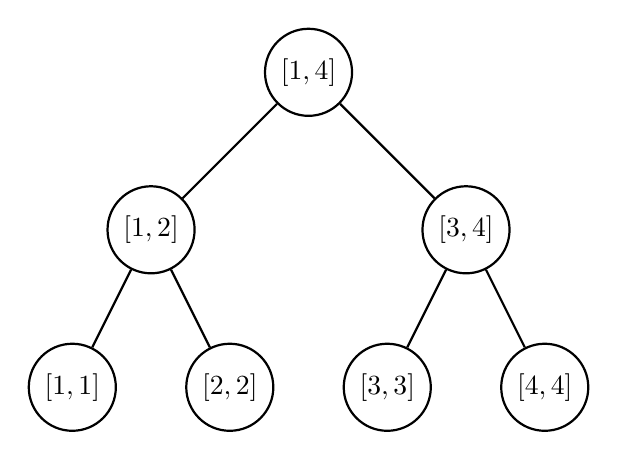
\begin{tikzpicture}
			\node[draw, circle, thick] (1) at (0,4) {$[1, 4]$};

			\node[draw, circle, thick] (2) at (-2,2) {$[1, 2]$};
			\node[draw, circle, thick] (3) at (2,2) {$[3, 4]$};

			\node[draw, circle, thick] (4) at (-3,0) {$[1, 1]$};
			\node[draw, circle, thick] (5) at (-1,0) {$[2, 2]$};
			\node[draw, circle, thick] (6) at (1,0) {$[3, 3]$};
			\node[draw, circle, thick] (7) at (3,0) {$[4, 4]$};

			\path[draw, thick] (1) -- (2);
			\path[draw, thick] (1) -- (3);
			\path[draw, thick] (2) -- (4);
			\path[draw, thick] (2) -- (5);
			\path[draw, thick] (3) -- (6);
			\path[draw, thick] (3) -- (7);
        \end{tikzpicture}
    \end{center}
\end{frame}

\begin{frame}[plain]{Drawn Segment Tree, $n = 7$}
	\begin{center}
		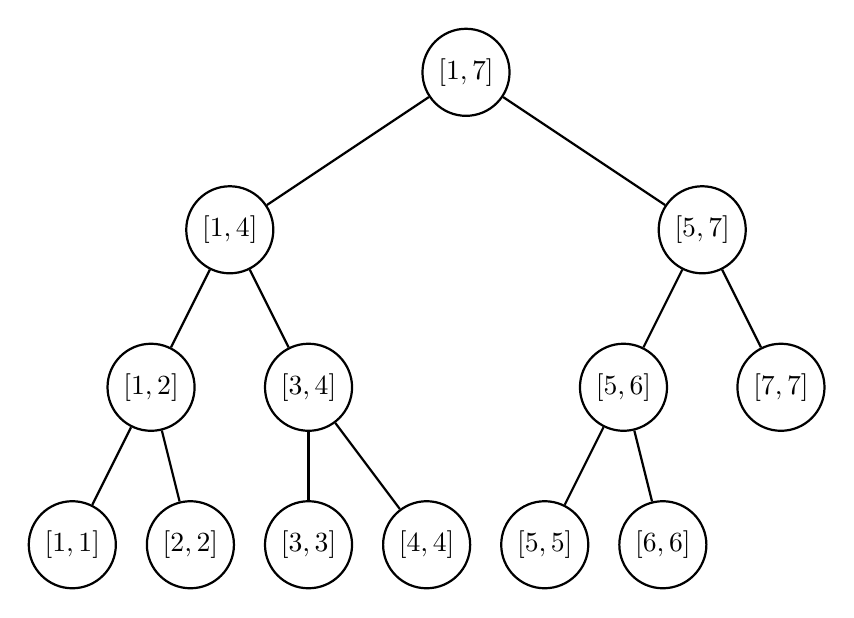
\begin{tikzpicture}
			\node[draw, circle, thick] (1) at (0,6) {$[1, 7]$};

			\node[draw, circle, thick] (2) at (-3,4) {$[1, 4]$};
			\node[draw, circle, thick] (3) at (3,4) {$[5, 7]$};

			\node[draw, circle, thick] (4) at (-4,2) {$[1, 2]$};
			\node[draw, circle, thick] (5) at (-2,2) {$[3, 4]$};
			\node[draw, circle, thick] (6) at (2,2) {$[5, 6]$};
			\node[draw, circle, thick] (7) at (4,2) {$[7, 7]$};

			\node[draw, circle, thick] (8) at (-5,0) {$[1, 1]$};
			\node[draw, circle, thick] (9) at (-3.5,0) {$[2, 2]$};
			\node[draw, circle, thick] (10) at (-2,0) {$[3, 3]$};
			\node[draw, circle, thick] (11) at (-0.5,0) {$[4, 4]$};
			\node[draw, circle, thick] (12) at (1,0) {$[5, 5]$};
			\node[draw, circle, thick] (13) at (2.5,0) {$[6, 6]$};

			\path[draw, thick] (1) -- (2);
			\path[draw, thick] (1) -- (3);
			\path[draw, thick] (2) -- (4);
			\path[draw, thick] (2) -- (5);
			\path[draw, thick] (3) -- (6);
			\path[draw, thick] (3) -- (7);
			\path[draw, thick] (4) -- (8);
			\path[draw, thick] (4) -- (9);
			\path[draw, thick] (5) -- (10);
			\path[draw, thick] (5) -- (11);
			\path[draw, thick] (6) -- (12);
			\path[draw, thick] (6) -- (13);
        \end{tikzpicture}
    \end{center}
\end{frame}

\begin{frame}[plain,fragile]{Segment Tree - Code}
    \begin{minted}[fontsize=\scriptsize]{cpp}
struct segment_tree {
    segment_tree *left, *right;
    int from, to, value;
    segment_tree(int from, int to)
        : from(from), to(to), left(NULL), right(NULL), value(0) { }
};

segment_tree* build(const vector<int> &arr, int l, int r) {
    if (l > r) return NULL;
    segment_tree *res = new segment_tree(l, r);
    if (l == r) {
        res->value = arr[l];
    } else {
        int m = (l + r) / 2;
        res->left = build(arr, l, m);
        res->right = build(arr, m + 1, r);
        if (res->left != NULL) res->value += res->left->value;
        if (res->right != NULL) res->value += res->right->value;
    }
    return res;
}
    \end{minted}
\end{frame}

\begin{frame}[plain]{Updates}
	\begin{center}
		\begin{tikzpicture}
			\only<all:1-2, 14-15, 24-> { \node[draw, circle, thick] (1) at (0,6) {\phantom{xxx}}; }
			\only<all:3-13, 16-23> { \node[draw, circle, thick, red] (1) at (0,6) {\phantom{xxx}}; }


			\only<all:1-3, 12-> { \node[draw, circle, thick] (2) at (-3,4) {\phantom{xxx}}; }
			\only<all:4-11> { \node[draw, circle, thick, red] (2) at (-3,4) {\phantom{xxx}}; }

			\only<all:1-16, 22-> { \node[draw, circle, thick] (3) at (3,4) {\phantom{xxx}}; }
			\only<all:17-21> { \node[draw, circle, thick, red] (3) at (3,4) {\phantom{xxx}}; }


			\only<all:1-> { \node[draw, circle, thick] (4) at (-4,2) {\phantom{xxx}}; }

			\only<all:1-4, 10-> { \node[draw, circle, thick] (5) at (-2,2) {\phantom{xxx}}; }
			\only<all:5-9> { \node[draw, circle, thick, red] (5) at (-2,2) {\phantom{xxx}}; }

			\only<all:1-> { \node[draw, circle, thick] (6) at (2,2) {\phantom{xxx}}; }

			\only<all:1-17, 20-> { \node[draw, circle, thick] (7) at (4,2) {\phantom{xxx}}; }
			\only<all:18-19> { \node[draw, circle, thick, red] (7) at (4,2) {\phantom{xxx}}; }


			\only<all:1-> { \node[draw, circle, thick] (8) at (-5,0) {\phantom{xxx}}; }

			\only<all:1-> { \node[draw, circle, thick] (9) at (-3.5,0) {\phantom{xxx}}; }

			\only<all:1-> { \node[draw, circle, thick] (10) at (-2,0) {\phantom{xxx}}; }

			\only<all:1-5, 8-> { \node[draw, circle, thick] (11) at (-0.5,0) {\phantom{xxx}}; }
			\only<all:6-7> { \node[draw, circle, thick, red] (11) at (-0.5,0) {\phantom{xxx}}; }

			\only<all:1-> { \node[draw, circle, thick] (12) at (1,0) {\phantom{xxx}}; }

			\only<all:1-> { \node[draw, circle, thick] (13) at (2.5,0) {\phantom{xxx}}; }

			\path[draw, thick] (1) -- (2);
			\path[draw, thick] (1) -- (3);
			\path[draw, thick] (2) -- (4);
			\path[draw, thick] (2) -- (5);
			\path[draw, thick] (3) -- (6);
			\path[draw, thick] (3) -- (7);
			\path[draw, thick] (4) -- (8);
			\path[draw, thick] (4) -- (9);
			\path[draw, thick] (5) -- (10);
			\path[draw, thick] (5) -- (11);
			\path[draw, thick] (6) -- (12);
			\path[draw, thick] (6) -- (13);


			\only<all:2-14> { \node at (-3,6) {\texttt{update(3, 7)}}; }
			\only<all:15-24> { \node at (-3,6) {\texttt{update(6, -12)}}; }
			\only<all:25-> { \node at (-3,6) {}; }

			\only<all:1-12> { \node at (0,6) {$40$}; }
			\only<all:13-22> { \node at (0,6) {$47$}; }
			\only<all:23-> { \node at (0,6) {$35$}; }

			\only<all:1-10> { \node at (-3,4) {$16$}; }
			\only<all:11-> { \node at (-3,4) {$23$}; }

			\only<all:1-20> { \node at (3,4) {$24$}; }
			\only<all:21-> { \node at (3,4) {$12$}; }

			\only<all:1-> { \node at (-4,2) {$5$}; }

			\only<all:1-8> { \node at (-2,2) {$11$}; }
			\only<all:9-> { \node at (-2,2) {$18$}; }

			\only<all:1-> { \node at (2,2) {$17$}; }

			\only<all:1-18> { \node at (4,2) {$7$}; }
			\only<all:19-> { \node at (4,2) {$-5$}; }

			\only<all:1-> { \node at (-5,0) {$3$}; }

			\only<all:1-> { \node at (-3.5,0) {$2$}; }

			\only<all:1-> { \node at (-2,0) {$9$}; }

			\only<all:1-6> { \node at (-0.5,0) {$2$}; }
			\only<all:7-> { \node at (-0.5,0) {$9$}; }

			\only<all:1-> { \node at (1,0) {$9$}; }

			\only<all:1-> { \node at (2.5,0) {$8$}; }
        \end{tikzpicture}
    \end{center}
\end{frame}

\begin{frame}[plain,fragile]{Updating a Segment Tree - Code}
    \vspace{40pt}
    \begin{minted}[fontsize=\scriptsize]{cpp}
int update(segment_tree *tree, int i, int val) {
    if (tree == NULL) return 0;
    if (tree->to < i) return tree->value;
    if (i < tree->from) return tree->value;
    if (tree->from == tree->to && tree->from == i) {
        tree->value = val;
    } else {
        tree->value = update(tree->left, i, val) + update(tree->right, i, val);
    }
    return tree->value;
}
    \end{minted}
\end{frame}

\begin{frame}[plain]{Querying}
	\begin{center}
		\begin{tikzpicture}
			\only<all:2-9> { \node at (-3,6) {\texttt{query(1, 7)}}; }
			\only<all:10-17> { \node at (-3,6) {\texttt{query(1, 2)}}; }

			\only<all:8> { \node at (-3,5.5) {\texttt{= 2 + 18 + 12}}; }
			\only<all:9> { \node at (-3,5.5) {\texttt{= 32}}; }
			\only<all:16> { \node at (-3,5.5) {\texttt{= 2 + 9}}; }
			\only<all:17> { \node at (-3,5.5) {\texttt{= 11}}; }



			\only<all:1-2, 4-10, 12-> { \node[draw, circle, thick] (1) at (0,6) {\phantom{xxx}}; }
			\only<all:3, 11> { \node[draw, circle, thick, red] (1) at (0,6) {\phantom{xxx}}; }


			\only<all:1-3, 5-11, 13-> { \node[draw, circle, thick] (2) at (-3,4) {\phantom{xxx}}; }
			\only<all:4, 12> { \node[draw, circle, thick, red] (2) at (-3,4) {\phantom{xxx}}; }

			\only<all:1-3, 10-> { \node[draw, circle, thick] (3) at (3,4) {\phantom{xxx}}; }
			\only<all:4> { \node[draw, circle, thick, red] (3) at (3,4) {\phantom{xxx}}; }
			\only<all:5-9> { \node[draw, circle, thick, blue] (3) at (3,4) {\phantom{xxx}}; }


			\only<all:1-4, 6-12, 14-> { \node[draw, circle, thick] (4) at (-4,2) {\phantom{xxx}}; }
			\only<all:5, 13> { \node[draw, circle, thick, red] (4) at (-4,2) {\phantom{xxx}}; }

			\only<all:1-4, 10-12, 14-> { \node[draw, circle, thick] (5) at (-2,2) {\phantom{xxx}}; }
			\only<all:5, 13> { \node[draw, circle, thick, red] (5) at (-2,2) {\phantom{xxx}}; }
			\only<all:6-9> { \node[draw, circle, thick, blue] (5) at (-2,2) {\phantom{xxx}}; }

			\only<all:1-> { \node[draw, circle, thick] (6) at (2,2) {\phantom{xxx}}; }

			\only<all:1-> { \node[draw, circle, thick] (7) at (4,2) {\phantom{xxx}}; }


			\only<all:1-> { \node[draw, circle, thick] (8) at (-5,0) {\phantom{xxx}}; }

			\only<all:1-5, 10-13, 18-> { \node[draw, circle, thick] (9) at (-3.5,0) {\phantom{xxx}}; }
			\only<all:6, 14> { \node[draw, circle, thick, red] (9) at (-3.5,0) {\phantom{xxx}}; }
			\only<all:7-9, 15-17> { \node[draw, circle, thick, blue] (9) at (-3.5,0) {\phantom{xxx}}; }

			\only<all:1-13, 18-> { \node[draw, circle, thick] (10) at (-2,0) {\phantom{xxx}}; }
			\only<all:14> { \node[draw, circle, thick, red] (10) at (-2,0) {\phantom{xxx}}; }
			\only<all:15-17> { \node[draw, circle, thick, blue] (10) at (-2,0) {\phantom{xxx}}; }

			\only<all:1-> { \node[draw, circle, thick] (11) at (-0.5,0) {\phantom{xxx}}; }

			\only<all:1-> { \node[draw, circle, thick] (12) at (1,0) {\phantom{xxx}}; }

			\only<all:1-> { \node[draw, circle, thick] (13) at (2.5,0) {\phantom{xxx}}; }

			\path[draw, thick] (1) -- (2);
			\path[draw, thick] (1) -- (3);
			\path[draw, thick] (2) -- (4);
			\path[draw, thick] (2) -- (5);
			\path[draw, thick] (3) -- (6);
			\path[draw, thick] (3) -- (7);
			\path[draw, thick] (4) -- (8);
			\path[draw, thick] (4) -- (9);
			\path[draw, thick] (5) -- (10);
			\path[draw, thick] (5) -- (11);
			\path[draw, thick] (6) -- (12);
			\path[draw, thick] (6) -- (13);

			\node at (0,6) {$35$};
			\node at (-3,4) {$23$};
			\node at (3,4) {$12$};
			\node at (-4,2) {$5$};
			\node at (-2,2) {$18$};
			\node at (2,2) {$17$};
			\node at (4,2) {$-5$};
			\node at (-5,0) {$3$};
			\node at (-3.5,0) {$2$};
			\node at (-2,0) {$9$};
			\node at (-0.5,0) {$9$};
			\node at (1,0) {$9$};
			\node at (2.5,0) {$8$};
        \end{tikzpicture}
    \end{center}
\end{frame}


\begin{frame}[plain,fragile]{Querying a Segment Tree - Code}
    \vspace{50pt}
    \begin{minted}[fontsize=\scriptsize]{cpp}
int query(segment_tree *tree, int l, int r) {
    if (tree == NULL) return 0;
    if (l <= tree->from && tree->to <= r) return tree->value;
    if (tree->to < l) return 0;
    if (r < tree->from) return 0;
    return query(tree->left, l, r) + query(tree->right, l, r);
}
    \end{minted}
\end{frame}

\begin{frame}[plain]{Segment Tree}
    \begin{itemize}
        \item<1-> Simple to use Segment Trees for $\min$, $\max$, $\gcd$, and other similar operators, basically the same code.
        \item<2-> Any associative operator will work.
        \item<3-> So any operator $f$ such that $f(a, f(b, c)) = f(f(a, b), c)$ for all $a, b, c$.
    \end{itemize}
\end{frame}

\begin{frame}[plain]{Example problem: Movie Collection}
    \begin{itemize}
        \item https://open.kattis.com/problems/moviecollection
    \end{itemize}
\end{frame}

\subsection*{Range updates and queries}

\begin{frame}[plain]{Range updates}
    \begin{itemize}
        \item<1-> So far, we have only allowed updates to affect a single element.
        \item<2-> Might want to update multiple elements simultaneously, iterating for each is expensive.
        \item<3-> Example: For all indices from $4$ to $7$ add $13$.
        \item<4-> Can we make use of our segmented structure to update all indices in range $[l, r]$?
        \item<5-> Lazy people tend to find efficient ways of doing all that \textbf{needs} to be done, but no more.
        \item<6-> After updating a value, there is no guarantee you will use the updated value afterwards.
        \item<7-> Idea: Be lazy and procrastinate changes until they are needed!
    \end{itemize}
\end{frame}

\begin{frame}[plain]{Lazy propagation}
    \begin{itemize}
        \item<1-> Add another variable for each node, storing the lazy value
        \item<2-> Follow same steps as querying in order to update, applying the update if the node is completely within the range.
        \item<3-> When making updates, do not change the original data variable, but rather the lazy variable.
        \item<4-> When looking at a node, apply the lazy value to the node
        \item<5-> After applying, push the lazy value to the two child nodes
        \item<6-> Reset the lazy value.
        \item<7-> Traverse to child nodes if needed.
    \end{itemize}
\end{frame}

\begin{frame}[plain]{Code example}
    See implementation example, for example \href{https://github.com/keppnisforritun/aflv_slides/tree/main/week7}{here}.
\end{frame}

\section*{Sparse Table}

\begin{frame}[plain]{Another $\log(n)$ idea}
    \begin{itemize}
        \item<1-> What if we tried something more akin to an array.
        \item<2-> Could we store $\log(n)$ amounts of data per element somehow?
        \item<3-> Yes! For each $i$ we can store the sum on the interval $[i, i + 2^j - 1]$ for $\log$ many $j$.
        \item<4-> Then to retrieve a sum from $i$ to $j$ we always take the biggest chunk we can that's stored at $i$, which will always be at least half.
        \item<5-> Then we continue until we reach $j$, moving $i$ along and collecting the results.
        \item<6-> This is what is known as a sparse table.
    \end{itemize}
\end{frame}

\begin{frame}[plain]{Sparse tables}
    \begin{itemize}
        \item<1-> Calculating all of these values takes $\mathcal{O}(n\log(n))$ because we can calculate the values in order of increasing $j$.
        \item<2-> Then when we calculate the sum of $[i, i + 2^j - 1]$ we just combine the earlier results of $[i, i + 2^{j-1} - 1]$ and $[i + 2^{j-1}, i + 2^j - 1]$.
        \item<3-> Querying takes $\mathcal{O}(\log(n))$, however updating is slow and difficult.
        \item<4-> Why would we then ever use this instead of segment trees?
    \end{itemize}
\end{frame}

\begin{frame}[plain]{Binary lifting}
    \begin{itemize}
        \item<1-> The reason might be is that with sparse tables we can do many things that segment trees can not because of how the results are combined.
        \item<2-> Let us consider binary lifting in particular.
        \item<3-> Suppose we have some function $f$ that rearranges the values $\{0, 1, \dots, n - 1\}$ and we get $q$ queries asking what happens to $x$ if we apply $f$ exactly $m$ times to $x$.
        \item<4-> The naïve solution is to calculate it every time, giving a time complexity of $\mathcal{O}(qm\mathcal{O}(f))$.
        \item<5-> How might we use sparse tables to do better?
    \end{itemize}
\end{frame}

\begin{frame}[plain]{Binary lifting ctd.}
    \begin{itemize}
        \item<1-> Let $f^{[y]}(x)$ denote the result of applying $f$ exactly $y$ times to $x$
        \item<2-> For each $i$ we store $f^{[2^j]}(i)$ as a sparse table
        \item<3-> Then we can compute these in increasing order of $j$, calculating $j = 1$ using $f$ itself and then for larger $j$ letting $f^{[2^j]}(x) = f^{[2^{j-1}]}(f^{[2^{j-1}]}(x))$
        \item<4-> Thus we can precompute the table in $\mathcal{O}(n(\mathcal{O}(f) + \log(n)))$ and each query takes $\mathcal{O}(\log(m))$, a much better time complexity
    \end{itemize}
\end{frame}

\begin{frame}[plain]{Sparse table example}
    \begin{center}
        \begin{tikzpicture}[scale=0.75]
            \draw[step=1,black,thin] (0,0) grid (12, 1);
            \node[align=left] at (13.5,0.5) {$j = 0$};
            \node at (0.5,0.5) {$7$};
            \node at (1.5,0.5) {$1$};
            \node at (2.5,0.5) {$6$};
            \node at (3.5,0.5) {$4$};
            \node at (4.5,0.5) {$8$};
            \node at (5.5,0.5) {$0$};
            \node at (6.5,0.5) {$9$};
            \node at (7.5,0.5) {$2$};
            \node at (8.5,0.5) {$2$};
            \node at (9.5,0.5) {$7$};
            \node at (10.5,0.5) {$1$};
            \node at (11.5,0.5) {$6$};

            \only<2-> {
                \draw[step=1,blue,thin] (0,1) grid (12, 2);
                \node[align=left] at (13.5,1.5) {\color{blue} $j = 1$};
            }
            \foreach \x in {3,4,...,13} {
                \only<\x> {
                    \draw[->, blue] ({0.5+\x-3}, 0.75) -- ({0.5+\x-3}, 1.25);
                    \draw[->, blue] ({1.25+\x-3}, 0.75) -- ({0.75+\x-3}, 1.25); 
                }
            }
            \foreach \x [count=\i] in {8, 7, 10, 12, 8, 9, 11, 4, 9, 8, 7, 6} {
                \pgfmathtruncatemacro{\onlyi}{\i+2}
                \only<\onlyi-> {
                    \node at ({-0.5+\i},1.5) {\color{blue} $\x$};
                }
            }

            \only<14> {
                \draw[->, blue] (11.5, 0.75) -- (11.5, 1.25);
            }

            \only<15-> {
                \draw[step=1,dark green,thin] (0,2) grid (12, 3);
                \node[align=left] at (13.5,2.5) {\color{dark green} $j = 2$};
            }
            \foreach \x in {3,4,...,12} {
                \only<15> {
                    \draw[->, dark green] ({0.5+\x-3}, 1.75) -- ({0.5+\x-3}, 2.25);
                    \draw[->, dark green] ({1.25+\x-2}, 1.75) -- ({0.75+\x-3}, 2.25); 
                }
            }
            \only<15> {
                \draw[->, dark green] (11.5, 1.75) -- (11.5, 2.25);
                \draw[->, dark green] (10.5, 1.75) -- (10.5, 2.25);
            }
            \foreach \x [count=\i] in {18, 19, 18, 21, 19, 13, 20, 12, 16, 14, 7, 6} {
                \only<15-> {
                    \node at ({-0.5+\i},2.5) {\color{dark green} $\x$};
                }
            }

            \only<16-> {
                \draw[step=1,dark yellow,thin] (0,3) grid (12, 4);
                \node[align=left] at (13.5,3.5) {\color{dark yellow} $j = 3$};
            }
            \foreach \x in {3,4,...,10} {
                \only<16> {
                    \draw[->, dark yellow] ({0.5+\x-3}, 2.75) -- ({0.5+\x-3}, 3.25);
                    \draw[->, dark yellow] ({1.25+\x}, 2.75) -- ({0.75+\x-3}, 3.25); 
                }
            }
            \only<16> {
                \draw[->, dark yellow] (11.5, 2.75) -- (11.5, 3.25);
                \draw[->, dark yellow] (10.5, 2.75) -- (10.5, 3.25);
                \draw[->, dark yellow] (9.5, 2.75) -- (9.5, 3.25);
                \draw[->, dark yellow] (8.5, 2.75) -- (8.5, 3.25);
            }
            \foreach \x [count=\i] in {37, 32, 38, 33, 35, 27, 27, 18, 16, 14, 7, 6} {
                \only<16-> {
                    \node at ({-0.5+\i},3.5) {\color{dark yellow} $\x$};
                }
            }

            \only<17> {
                \node at (5, 5) {\texttt{query(1, 8) = 19 + 9 + 2}};
                \draw[red, very thick] (1, 2) -- (2, 2) -- (2, 3) -- (1, 3) -- cycle;
                \draw[red, very thick] (5, 1) -- (6, 1) -- (6, 2) -- (5, 2) -- cycle;

                \draw[red, very thick] (1, 0) -- (5, 0) -- (5, 1) -- (1, 1) -- cycle;
                \draw[red, very thick] (5, 0) -- (7, 0) -- (7, 1) -- (5, 1) -- cycle;
                \draw[red, very thick] (7, 0) -- (8, 0) -- (8, 1) -- (7, 1) -- cycle;
            }

            \only<18> {
                \node at (5, 5) {\texttt{query(0, 9) = 37 + 9}};
                \draw[red, very thick] (0, 3) -- (1, 3) -- (1, 4) -- (0, 4) -- cycle;
                \draw[red, very thick] (8, 1) -- (9, 1) -- (9, 2) -- (8, 2) -- cycle;

                \draw[red, very thick] (0, 0) -- (8, 0) -- (8, 1) -- (0, 1) -- cycle;
                \draw[red, very thick] (8, 0) -- (10, 0) -- (10, 1) -- (8, 1) -- cycle;
            }

        \end{tikzpicture}
    \end{center}
\end{frame}

\begin{frame}[plain]{Example problem: Stikl}
    \begin{itemize}
        \item https://open.kattis.com/problems/stikl
    \end{itemize}
\end{frame}

\end{document}
